\section{Zur Verfügung gestellte Hardware des Autos}
\label{sec:grundlegendesHW}

Die Basis der zur Verfügung stehenden Hardware, also Chassis, Motoren, Servo, etc. sind handelsübliche Modellautos. Dabei besteht das Auto aus zwei Schichten. Die Basis bildet ein 16Bit Mikrocontroller der MB96300-Serie von \textit{Fujitsu Microelectronics} (heute: \textit{Cypress Semiconductor Corporation}). Die zweite Schicht der Hardware des Autos besteht aus einem vollwertigen Einplatinencomputer mit Quadcore-Prozessor, SSD-Speicher uvm. Der Mikrokontroller ist in der zu diesem Semester upgegradeten Hardware nur noch zur Vermittlung der Werte von Sensorik und Aktorik zwischen Hauptplatine und Peripherie zuständig. Somit hatten wir eine vollwertige API zur Hardware, sodass keine Software für Schnittstellen oder Treiber implementiert werden musste und (fast) keine Veränderungen am Mikrocontroller vorgenommen werden mussten. Als Sensoren stehen Hall-Sensoren an den Rädern, ein Liniensenor, eine USB-Webcam, sowie drei Ultraschallsensoren (rechts, links und vorne) zur Verfügung. Angesteuert wird die Lenkung des Modellautos über einen Servo. Der Antrieb des Autos ist durch Gleichstrommotoren, die durch einen Fahrtregler fast stufenlos angesteuert werden können, realisiert. Beides wird durch ein pulsweitenmoduliertes Signal vom Mikrokontroller gesteuert. Zudem ist ein WLAN-Modul integriert, sodass es möglich ist, auf das Auto per Ad-hoc-Verbindung zuzugreifen. 

\begin{figure}[htbp] 
	\centering
	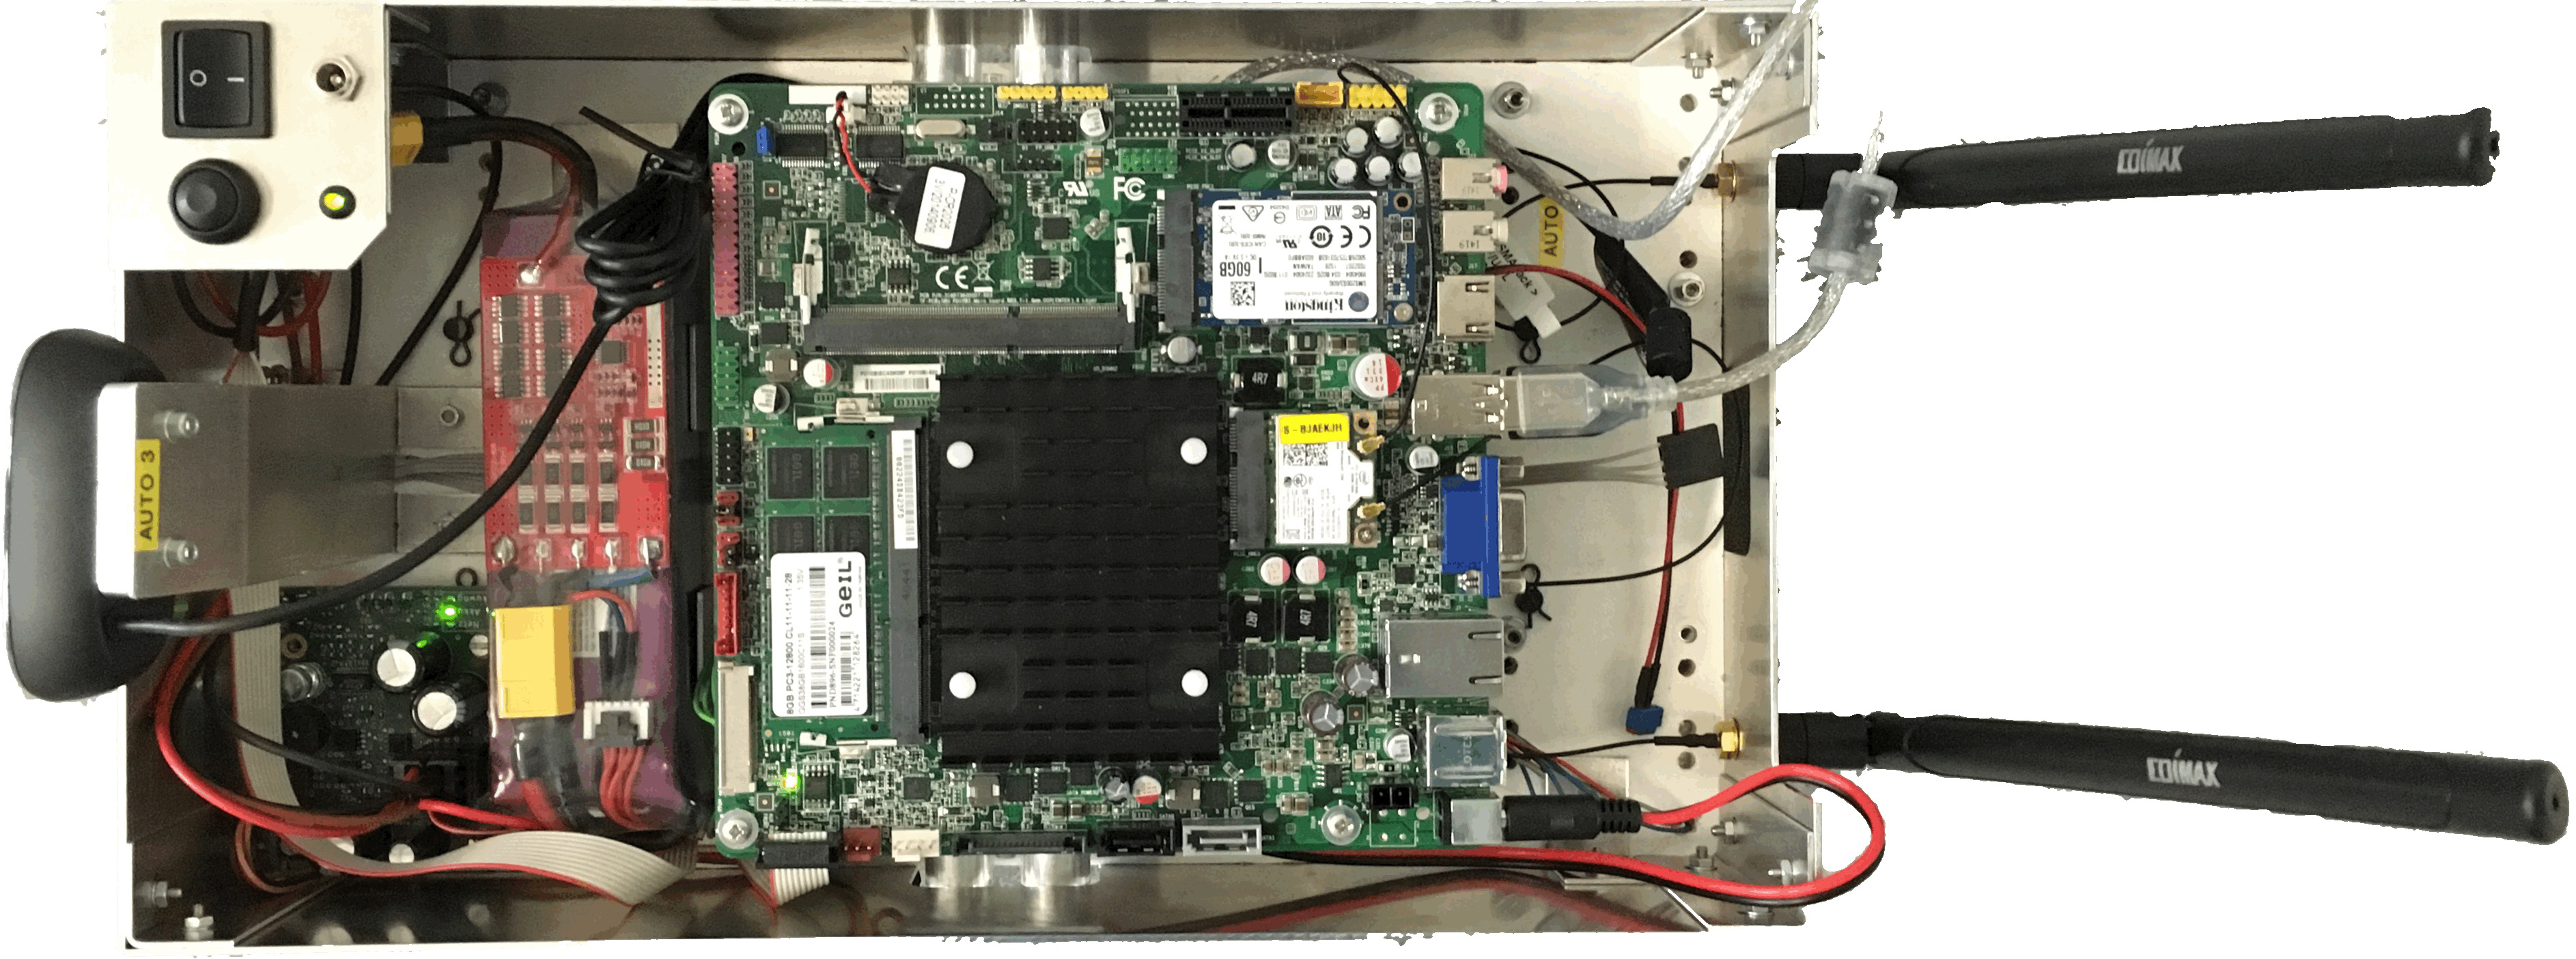
\includegraphics[width=350pt]{images/Animauto.jpg}
	\caption{Das Auto}
	\label{fig:DasAuto}
\end{figure}

Die Software auf dem Mikrokontroller, die zur Kommunikation zwischen der Anwendungssoftware und der Sensorik bzw. Aktorik zuständig ist, ist bereits vorimplementiert. Durch die so zur Verfügung gestellte API war eine einfache Nutzung der Hardware möglich. Jedoch war dadurch auch unklar, inwieweit die Signale der Sensorik manipuliert wurden. Die Ultraschallsensoren waren zu Beginn auf cm-Auflösung gestellt, was zu ungenauen Sensorwerten führte. Die abbildbare Tiefe betrug etwa 20cm bis 3m bei vielen Ausreißern und Diskrepanzen durch eine niedrige Auflösung. Um bessere Werte zu erhalten, haben wir auf dem Mikrokontroller von cm-Werte auf Mikrosekunden-Werte umgestellt. Dazu war es notwendig, die dafür zuständige Variable im Code des Mikrokontrollers von 0x51 auf 0x52 zu inkrementieren. Dies hat die Genauigkeit, sowie den Messbereich auf ca. 5m erhöht.